\documentclass[12pt,a4paper]{article}
\usepackage[margin=2cm]{geometry}
\usepackage{xeCJK}
\usepackage{fontspec}
\setCJKmainfont{Noto Serif CJK TC}[Script=CJK]
\usepackage{amsmath,amssymb}
\usepackage{bm}
\usepackage{graphicx}
\usepackage{fancyhdr}
\setlength{\headheight}{14.5pt}
\addtolength{\topmargin}{-2.5pt}
\usepackage{hyperref}
\usepackage{listings}
\usepackage{enumitem}
\usepackage{titlesec}
\usepackage{caption}
\usepackage{float}
\usepackage{indentfirst}
\usepackage{booktabs}
\setlength{\parindent}{2em}
\pagestyle{fancy}
\fancyhf{}
\cfoot{\thepage}
\linespread{1.3}
\usepackage{tikz}
\usetikzlibrary{arrows.meta, positioning}
\usepackage{cite}

\title{暑期專題報告書\\\large 肺部電腦斷層掃描之非小細胞癌 PD-L1 表現預測:\\結合多任務自監督學習與生成對抗網路}
\author{作者:戴偉璿}
\date{August 2025} 

\begin{document}

\rhead{2025 暑期專題報告書}
\lhead{肺部電腦斷層掃描之非小細胞癌 PD-L1 表現預測}

\maketitle

\newpage
\tableofcontents
\newpage

\section*{摘要}

醫學影像的稀缺 一直以來都是機器學習輔助診斷的一大挑戰,在資料量不足的狀況下,模型的收斂尤為困難,使其準確率不佳或是缺乏泛化能力。近年來,自監督學習(Self-supervised Learning)儼然成為解決資料稀缺問題的重要方法,藉由模型自己將未標記資料轉化為有用的特徵表示,能夠在少量標記資料的情況下顯著提升模型性能,而多任務自監督學習(Multi-task Self-supervised Learning)方法,通過同時學習多個相關任務,能夠進一步增強模型的表徵學習能力。藉由上游任務的預訓練取得更好的特徵表示,將權重微調到下游任務,使其能夠在資料量不足的情況下,提升模型的準確率。

本專題參考周姵妤學姐的碩士論文「肺部電腦斷層掃描之非小細胞癌 PD-L1 表現預測:結合遮蓋圖像模型與生成對抗網路」,使用大量由對抗神經網路(GAN)生成的 CT 影像進行預訓練,並在微調階段使用真實的醫學影像進行訓練。該模型結合了自監督重建、腫瘤分割與分類任務,在低資料條件下有效提升了 PD-L1 表現的預測準確率。本專題將在此基礎上進行改良,嘗試加入對比學習模組、模型集成策略,以期進一步提升 PD-L1 表現預測的準確率。

\section{緒論}

\subsection{研究背景(資料來源:周姵妤學姐碩士論文)}

據統計,肺癌是全球癌症相關死亡的主要原因之一。肺癌分成兩種:非小細胞肺癌(Non-small-cell lung carcinoma, NSCLC)與小細胞癌(Small-cell lung carcinoma, CSLC),其中 NSCLC 佔所有肺癌的 85\% 以上。由於肺癌的早期症狀不明顯,許多患者在診斷時已經處於晚期,這使得肺癌的治療變得更加困難,五年存活率依擴散程度介於6~33\%之間。

以往針對晚期 NSCLC 的治療較為受限,主要依賴化學療與放射治療。然而,化學治療的手段缺乏單一性,正常的細胞亦容易受到傷害,患者在接受治療的同時亦要承擔嚴重的副作用。治療時需要考量患者身體的耐受度來權衡治療的強度,這使得過往化學治療的效果極其有限,僅能達到 5\% 以下的五年存活率。

為改善過往缺乏專一性的治療,近年來 NSCLC 的治療著重在能針對腫瘤細胞進行控制、有效減緩病情的療法。隨研究進展,更精準的標靶藥物出現,其主要藉由藥物以抑制突變腫瘤基因,針對突變基因來擊殺癌細胞,這種具有基因單一性的機制使標靶治療的副作用相較於化學治療來的小,並有效改善患者 progression-free survival(PFS)的時間長度

標靶藥物的優點在於針對性強,能精準攻擊具有特定基因突變的腫瘤細胞。然而,這也是它的限制:僅對攜帶該突變(如 EGFR 基因突變)的患者有效,且主要用於肺腺癌等特定亞型。對於沒有 EGFR 突變或不屬於這些亞型的 NSCLC 患者,傳統標靶藥物效果有限。免疫檢查點抑制劑(Immune Checkpoint Inhibitors, ICIs)的出現帶來了突破。ICIs 通過阻斷 T 細胞上的 PD-1 與腫瘤細胞上的 PD-L1 的結合,解除免疫抑制,使 T 細胞重新啟動並攻擊腫瘤細胞。此種免疫療法對患者的負擔小於傳統的化學療法,也沒有標靶藥物的限制,能夠針對更廣泛的 NSCLC 患者,能有效改善 PFS 以及患者的存活率。

然而,此種免疫療法仍有其限制。免疫療法的原理是隔斷 PD-1 與 PD-L1 的結合,解除免疫抑制,使 T 細胞重新啟動並攻擊腫瘤細胞,因此細胞表面的 PD-L1 會直接影響治療的結果,PD-L1 的表現量是免疫治療中一個重要的生物標記,常用以評估 NSCLC 患者是否適合接受 PD-1/PD-L1 抑制劑。研究顯示,PD-L1 表現高的患者對免疫治療的反應較好,而 PD-L1 表現低的患者則可能需要聯合治療或非免疫療法。因此,準確預測 PD-L1 的表現量對於選擇合適的治療方案至關重要。為了克服現行 PD-L1 檢測方法的侷限,並提升表達量判讀的精確性,本研究引入電腦輔助診斷技術(Computer aided diagnosis, CAD)進行 PD-L1 分類分析,以期為臨床決策提供更可靠的依據。

以下是 PD-L1 表現的兩個例子,
50\% 是 NSCLC 中 PD-L1 表現的高低分界,>50\% 表示高表現,適合單藥免疫治療,預後較好;
<50\% 表示低表現,需聯合治療或非免疫療法,預後較差
\begin{figure}[H]
  \centering
  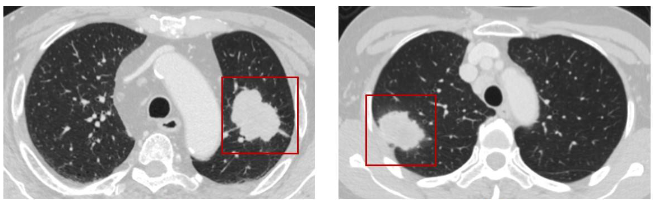
\includegraphics[width=0.8\textwidth]{src/image1.png}
  \centering
  \caption{左:PD-L1 表現>50\%;右:PD-L1 表現<50\%\\圖片來源:周姵妤學姐碩士論文}
  \label{fig:pdl1-examples}
\end{figure}

\subsection{挑戰與研究動機}

隨著醫學影像技術的進步,肺部電腦斷層掃描(CT)已成為非小細胞肺癌診斷的重要工具,但遇到了新的挑戰:樣本數量不足。
相較於其他領域,醫學影像的取得尤為困難,
不只是因為需要專業的醫療設備與人員,還因為涉及患者隱私與倫理問題。
因此,如何在有限的資料條件下,準確預測 PD-L1 表現並且盡可能提昇模型的泛化能力,
成為一個亟待解決的問題。

近年來,自監督學習(Self-supervised Learning)的發展為解決資料稀缺問題提供了新的思路。
自監督學習通過從未標記的資料中學習有用的特徵表示,能夠在少量標記資料的情況下,
顯著提升模型性能。特別是多任務自監督學習(Multi-task Self-supervised Learning)方法,
通過同時學習多個相關任務,能夠進一步增強模型的表徵學習能力。

周姵妤學姐的碩士論文:「肺部電腦斷層掃描之非小細胞癌 PD-L1 表現預測 :
結合遮蓋圖像模型與生成對抗網路」中提出了一種基於 Masked autoencoder (MAE)
模型改良後的多模態模型 MTMAE , MAE 模型是一種自監督學習方法,
通過遮蔽部分輸入影像來學習有效的特徵表示。
學姐使用了實驗室之前研究出的 GAN 生成 CT 影像對模型進行預訓練,
並在微調階段使用真實的醫學影像進行訓練。該模型
結合了自監督重建、腫瘤分割與分類任務,
在低資料條件下有效提升了 PD-L1 表現的預測準確率。基於該模型的潛力,
我想嘗試看看這個方法能否有進一步改進的空間。

\section{研究目標}
\begin{enumerate}
  \item 建立以 MTMAE 為基礎之 PD-L1 表現預測模型
  \item 探討加入對比學習對自監督表徵學習的增強效果。
  \item 在ViT encoder 中嵌入 GNN,建構 patch 間關聯性以提升特徵整合能力。
  \item 評估多模型集成(ensemble)策略對預測穩定性與泛化能力的影響。
\end{enumerate}

\section{研究方法}
本研究將基於周姵妤學姐的碩士論文所提出的 MTMAE 模型進行改良,
模型核心為 Multi-task Masked Autoencoder(MTMAE) 。由於
影像資料的缺乏,我們先使用 GAΝ 生成批量的影像,對模型進行預訓練,接下來再使用
真正的醫學影像進行微調。

\subsection{實驗材料}

本專案使用來自於台大醫院、台大醫院新竹分院、台大醫院雲林分院提供之非小細胞肺癌患者 CT 與 PD-L1 標記資料做為輸入資料。本研究總共蒐集 188 例病患,其中 PD-
L1 expression ≥ 50\%(+)有 49 例,PD-L1 expression < 50\% (−)有 139 例。下表紀錄了患者的年齡、性別、病理分類以及肺癌分期:

\begin{table}[h]
\centering
\begin{tabular}{lcccc}
\toprule
 & Total & PD-L1 $\geq 50\%$ & PD-L1 $< 50\%$ & p-value \\
\midrule
Age & 67 & 66 & 68 & 0.238 \\
\midrule
\textbf{Gender} & & & & 0.065 \\
\quad M & 105 & 36 & 69 & \\
\quad F & 83 & 13 & 70 & \\
\midrule
\textbf{Histopathology} & & & & 0.781 \\
\quad ADC & 126 & 28 & 98 & \\
\quad SCC & 30 & 8 & 22 & \\
\quad Others & 32 & 13 & 19 & \\
\midrule
\textbf{Stages} & & & & 0.246 \\
\quad I & 23 & 3 & 20 & \\
\quad II & 11 & 2 & 9 & \\
\quad III & 30 & 11 & 19 & \\
\quad IV & 124 & 33 & 91 & \\
\bottomrule
\end{tabular}
\end{table}
\newpage
此外,為了解決資料稀缺問題,本專案也會使用實驗室先前所開發之 Gabor-GAN 模型,使用公開資料庫
LIDC-IDRT(Lung Image Database Consortium and Image Database Resource Initiative) 生成 518,064 張2D的樣本。

使用 GAN 生成的影像來訓練模型常面臨真實性的爭議,能夠生成準確的肺結節影像是關鍵。
為了控制生成影像的真實性(結核的大小以及形狀),我們使用結節分割標記引導生成。
流程包括:首先分割肺結節與肺實質背景,將背景與分割 mask 輸入 GAN,訓練生成肺結節樣本。
Gabor-loss GAN 使用 CNN 架構,訓練時除了真偽分類損失,還透過 Gabor filter 計算濾波特徵的損失(Gabor-loss),增強結節紋理並避免過擬合。
訓練完成後,使用肺部組織分割演算法提取肺實質背景,選取 64$\times$64$\times$64 的 VOI 作為輸入,將真實結節標記置於中間,
排除與肺壁、心臟等重疊的區域,並確保標記體積保留 80\% 以上。最後用高斯濾波器和平滑處理優化結節與背景的邊界。

藉由以上複雜的生成流程,我們期許能獲得高品質、高準確率的肺結節影像,增加模型預測的準確率。

\newpage
\subsection{參考的模型}

\subsubsection{MIM 概念}

2018年, Devlin 等人提出了 BERT(Bidirectional Encoder Representations from Transformers)模型,這是一種基於 Transformer 架構的自監督學習方法。BERT 通過遮蔽部分輸入文本並且完成重建任務以學習有效的特徵表示,將其預訓練的 encoder 應用在許多 downstream 任務上,取得了顯著的效果。BERT 的成功啟發了許多後續的研究,特別是在影像領域。

隨後,這一思想被擴展到影像領域,形成了遮蓋圖像模型(Masked Image Model, MIM)的概念。2021年, Bao 等人提出了 BEiT 架構,將 BERT 的 SSL 方法應用在影響處理上,成功開發了一種適用於影響的 MIM 模型。同樣的,He 等人提出了 MAE(Masked Autoencoder)模型,結合了 autoencoder 與 MIM 的思想,通過遮蔽部分輸入影像來學習有效的特徵表示。MAE 模型在多個影像分類任務上取得了優異的效果,顯示了 MIM 方法在影像處理上的潛力。

\begin{figure}[H]
  \centering
  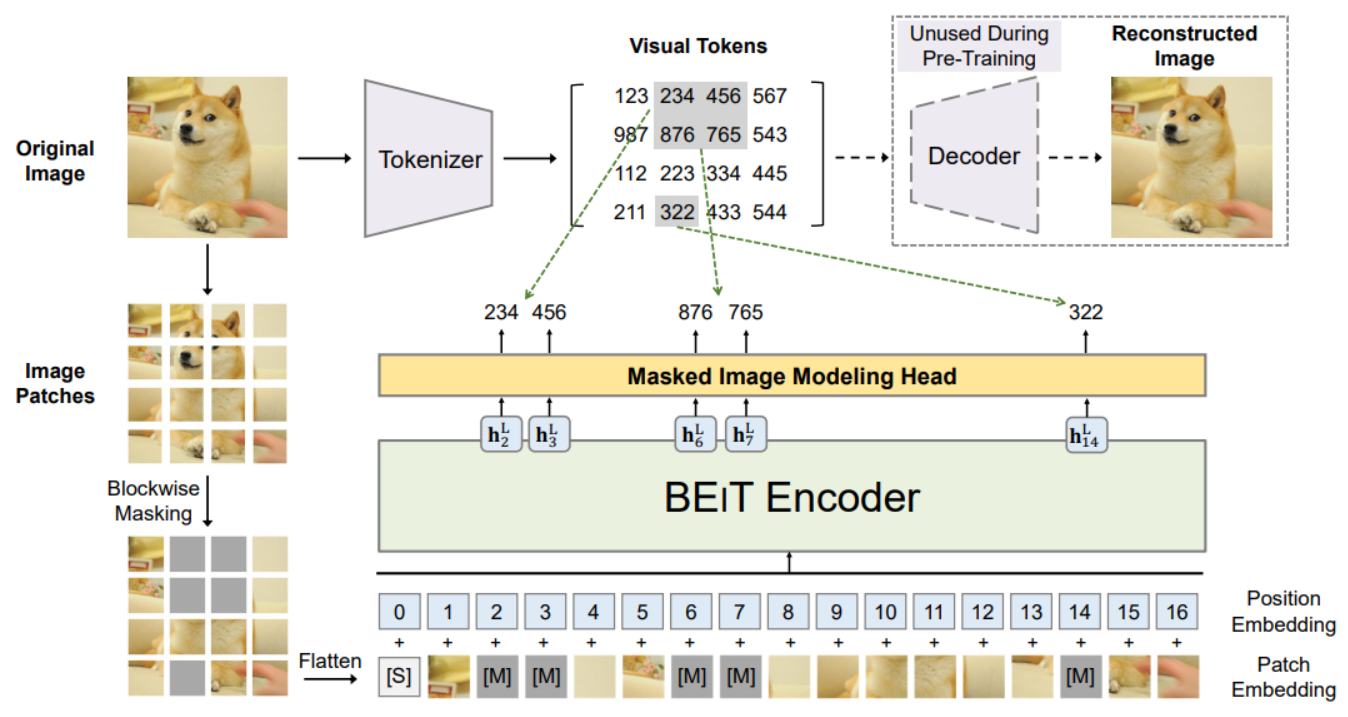
\includegraphics[width=0.8\textwidth]{src/BEiT.png}
  \centering
  \caption{BEiT 模型架構圖。\\圖片來源:https://arxiv.org/pdf/2106.08254}
  \label{fig:beit-architecture}
\end{figure}


MIM模型的訓練過程包含兩個部份:預訓練(pre-training)以及微調(fine-tuning)。在預訓練的階段中,對圖像進行隨機遮蓋,要求模型重建被遮蓋的部分,比較還原結果與真實圖像計算損失函數以優化權重。這一過程使模型學會了如何從部分信息中推斷出完整的圖像特徵,從而獲得有效的特徵表示。在微調階段,利用少量有標記的資料對預訓練得到的 encoder 進行微調,使其能進行如圖像分類、物體檢測等的下游任務。此 transfer learning 的過程使得模型能夠在少量標記資料的情況下,仍然達到較高的預測準確率。

\newpage
\subsubsection{MAE 模型}

MAE 本質上是一種特定的 MIM 實現方式,一樣是分成預訓練以及微調兩個階段。在預訓練的時候,模型將輸入的圖片隨機遮罩,並使用 autoencoder 嘗試將其還原。為了讓模型學習到完整的紋理以及特徵表示,使其無法透過簡單的差分重建被遮蓋的部份,遮蓋的比例極高(根據 He 等人在 MAE 模型中的實驗,遮蓋比例達到 75\%有最好的效果),這樣能夠強迫模型學習到更全面的特徵表示。在微調階段,使用少量帶有標記的資料讓模型能快速適應各式不同的下游任務。
MAE 模型的架構如下圖所示:

\begin{figure}[H]
  \centering
  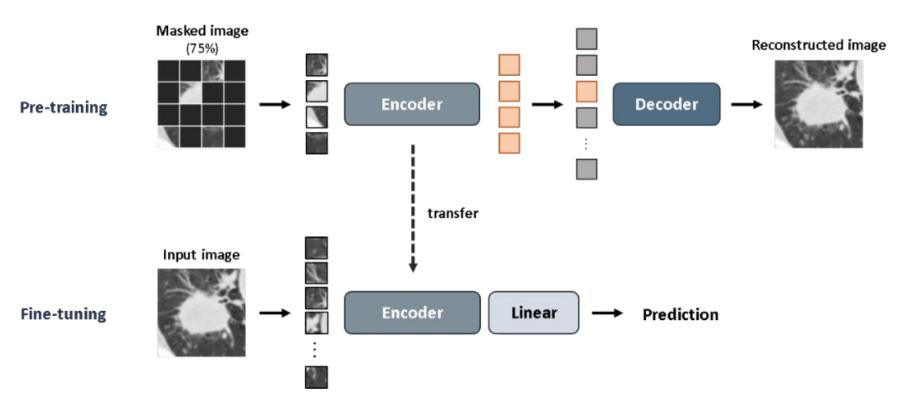
\includegraphics[width=0.8\textwidth]{src/MAE.png}
  \centering
  \caption{MAE 模型架構圖。\\圖片來源:周姵妤學姐碩士論文}
  \label{fig:MAE-architecture}
\end{figure}

下圖是一個使用 MAE 重建遮罩圖像的例子,左圖是原始影像;中圖是原始影像加上 75\% 的隨機遮罩;右圖是模型重建的結果。這組圖片是 pretrain 任務中進行到第 200 個 epoch 時的結果,此時模型已經學會了如何從部分信息中推斷出完整的圖像特徵。

\begin{figure}[H]
  \centering
  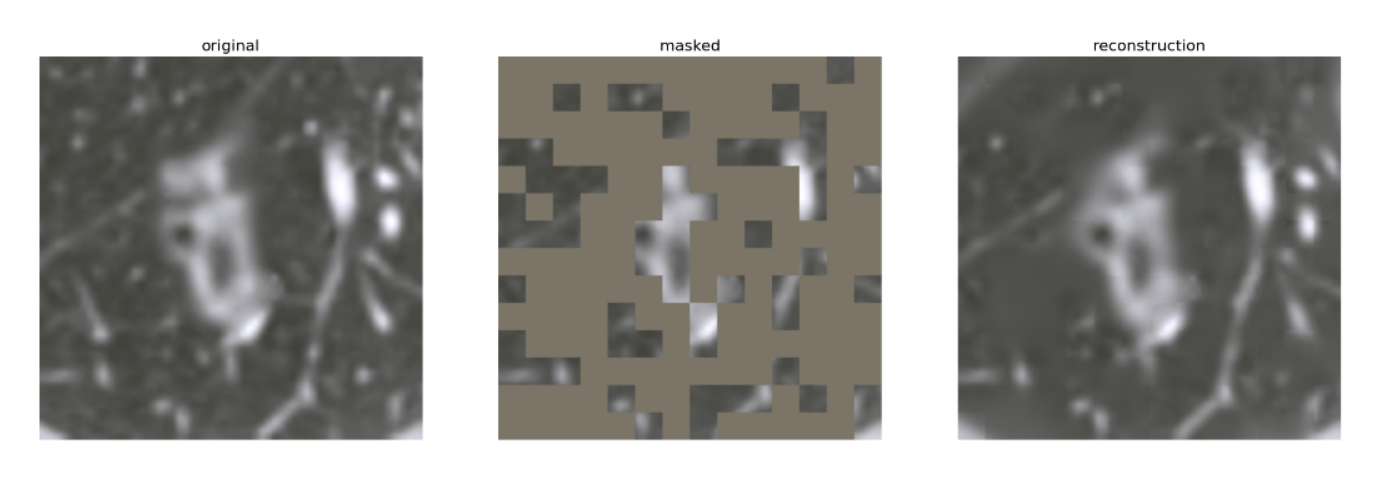
\includegraphics[width=0.6\textwidth]{src/MAE_example.png}
  \centering
  \caption{MAE 重建的範例。}
  \label{fig:MAE_example-architecture}
\end{figure}

\newpage
\subsubsection{MTMAE 模型}

周姵妤學姐在碩士論文中提出的 MTMAE 模型,基於 MAE 模型進行改良,將其應用於肺部 CT 影像的 PD-L1 表現預測任務。和自然的影像不同,肺部的 CT 影像中目標腫瘤大小各異,且與周圍的血管、組織等具有相同的灰度值,容易對干擾模型學習。然而,若是單純的去除背景,又可能會損失有用的資訊,因此學姐在 MTMAE 模型中結合了影像分割任務以及影像重建的任務,採用多任務學習的方式,提升模型的效能。

MTMAE 模型在預訓練階段使用大量由 GAN 生成的 CT 影像,同時進行影像分割以及重建的任務以學習特徵;在微調階段,使用預訓練得到的 encoder 加入 ViT 模型中,以預測 PD-L1 的表現。以下是 MTMAE 模型的架構圖:

\begin{figure}[H]
  \centering
  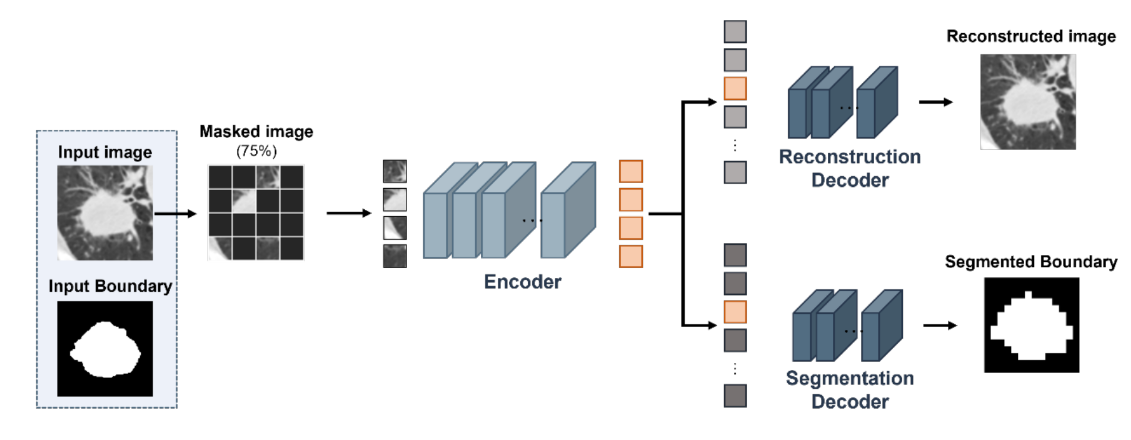
\includegraphics[width=0.8\textwidth]{src/MTMAE.png}
  \centering
  \caption{MTMAE 模型架構圖。\\圖片來源:周姵妤學姐碩士論文}
  \label{fig:MTMAE-architecture}
\end{figure}

\subsubsection{SimLR 模型}
自監督學習在近年來分成了兩大類方法:遮罩影像模型以及對比學習(Contrastive Learning, CL)。對比學習的核心概念是學習一個 embedding 空間,使相似的樣本接近,不相似樣本遠離。

SimCLR(Simple Framework for Contrastive Learning of Visual Representations)是 Chen 等人在 2020 年提出的自監督學習框架。SimCLR 的核心思想是通過對比學習來學習視覺表示,具體來說,它對同一張圖像應用不同的資料增強(data augmentation)方法生成正樣本對,並將不同圖像視為負樣本,通過最大化正樣本對之間的相似度、最小化負樣本對之間的相似度來學習有效的特徵表示。


\begin{figure}[H]
\small
    \centering
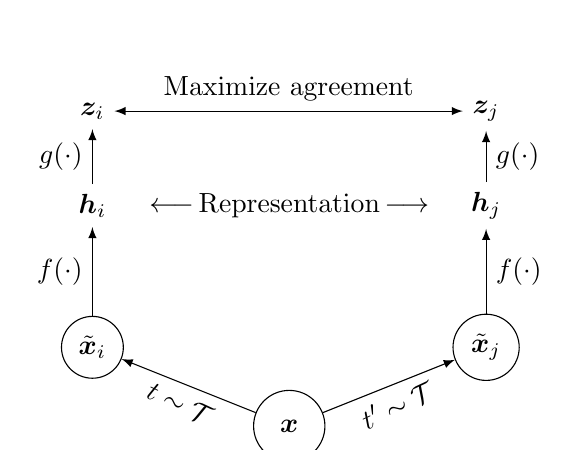
\begin{tikzpicture}
    \node at (0,1.8) (h) {$\longleftarrow\,$Representation$\,\longrightarrow$};
    \node[draw, circle] at (0,-1) (x) {$\,~\bm{x}~\,$};
    \node[draw, circle] at (-2.5,0) (x1) {$\tilde{\bm{x}}_i$};
    \node[draw, circle] at (2.5,0) (x2) {$\tilde{\bm{x}}_j$};
    \node at (-2.5,1.8) (h) {$\bm h_i$};
    \node at (2.5,1.8) (c) {$\bm h_j$};
    \node at (-2.5,3) (hh) {$\bm z_i$};
    \node at (2.5,3) (cc) {$\bm z_j$};
    \path[->] 
        (x)  edge [>=latex] node[below,rotate=-25] {$t\sim\mathcal{T}$} (x1)
        (x)  edge [>=latex] node[below,rotate=25] {$t'\sim \mathcal{T}$} (x2)
        (x1)  edge [>=latex] node[left,rotate=0] {$f(\cdot)$} (h)
        (x2)  edge [>=latex] node[right,rotate=0] {$f(\cdot)$} (c)
        (h)  edge [>=latex] node[left,rotate=0] {$g(\cdot)$} (hh)
        (c)  edge [>=latex] node[right,rotate=0] {$g(\cdot)$} (cc);
    \path[<->]
        (hh)  edge [>=latex] node[above,rotate=0] {Maximize agreement} (cc);
    \end{tikzpicture}
    \caption{SimLR 架構圖}
    \label{fig:simLR-framework}
\end{figure}


SimCLR 的優勢在於其簡潔性和有效性,不需要特殊的網路架構或記憶庫機制,僅通過資料增強和對比學習就能學習到高品質的視覺表示。然而,SimCLR 需要較大的批次大小才能獲得足夠的負樣本,這在醫學影像等資料稀缺的領域中可能成為限制。

\subsubsection{GCMAE 模型}
雖然 MAE 在圖像重建與表徵學習上取得了顯著的效果,但重建結果主要依賴局部資訊,容易忽略圖像中全域(global)的語意結構。為了進一步提升特徵表徵的品質,Quan 等人提出了 GCMAE(Global-Context Masked Autoencoder)模型,其核心思想是在 MAE 的基礎上引入全域上下文訊息,讓模型在重建被遮蔽區域時不僅依靠鄰近的局部特徵,也能參考整體圖像的語意分佈。以下是 GCMAE 模型的架構圖:

\begin{figure}[H]
  \centering
  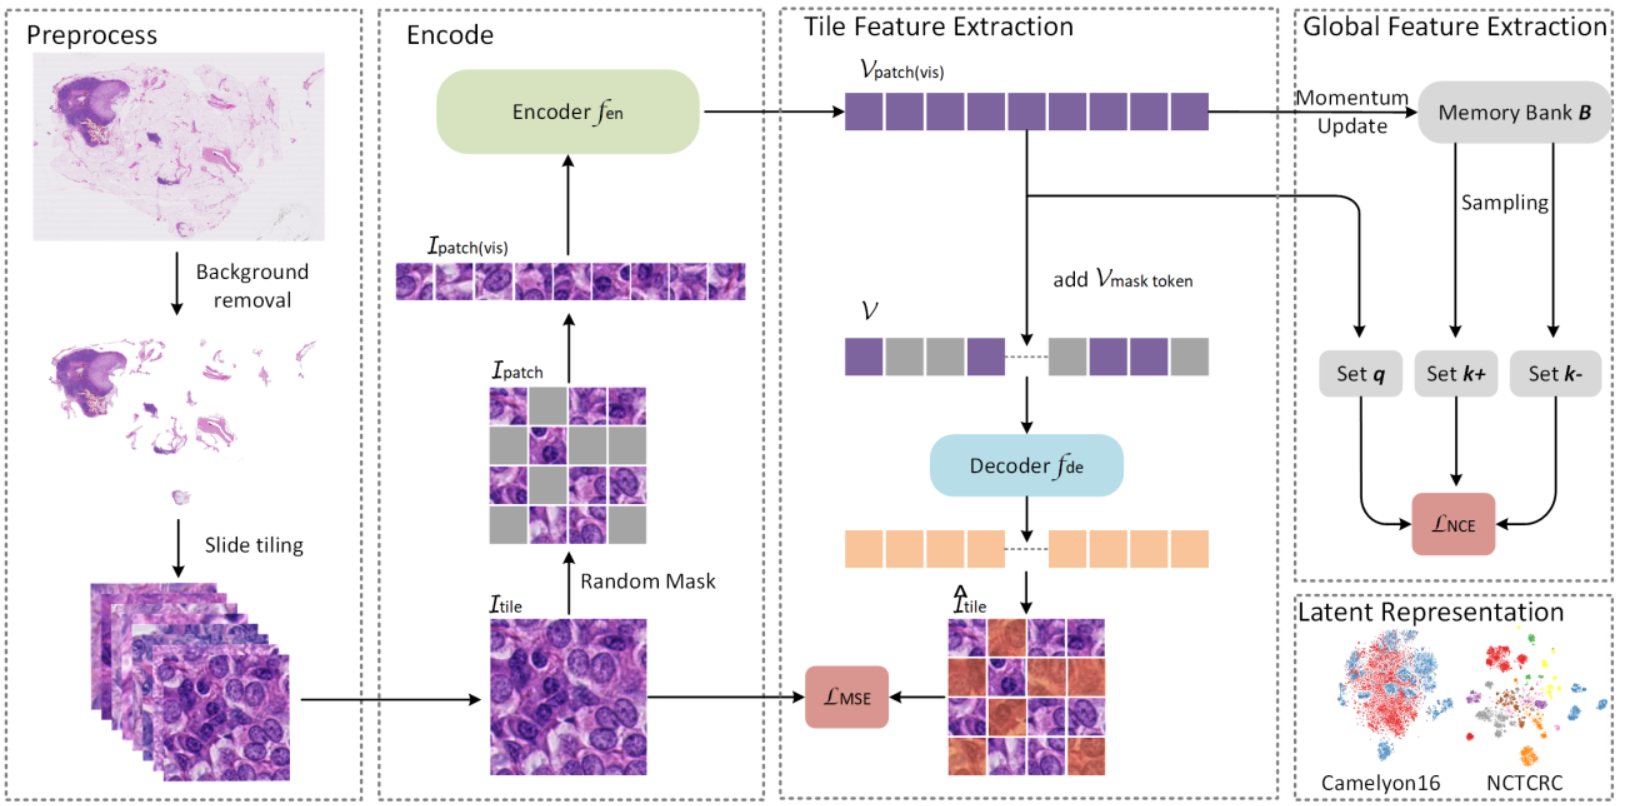
\includegraphics[width=0.8\textwidth]{src/GCMAE.png}
  \centering
  \caption{GCMAE 模型架構圖。\\圖片來源:https://arxiv.org/pdf/2205.09048}
  \label{fig:GCMAE-architecture}
\end{figure}

\newpage
\subsubsection{CMAE 模型}
Huang 等人在 2022 年提出了 CMAE(Contrastive Masked Autoencoder)模型,這是一種結合了對比學習與遮蔽自監督學習的模型。CMAE 利用孿生神經網路,以不對稱的框架同時進行圖像重建任務以及對比學習的任務。雖然說 CMAE 主要是以學習自然界的圖像為主(GCMAE 的目的是處理醫學影像),但其孿生網路的架構也值得借鑒。以下是 CMAE 的架構圖:

\begin{figure}[H]
  \centering
  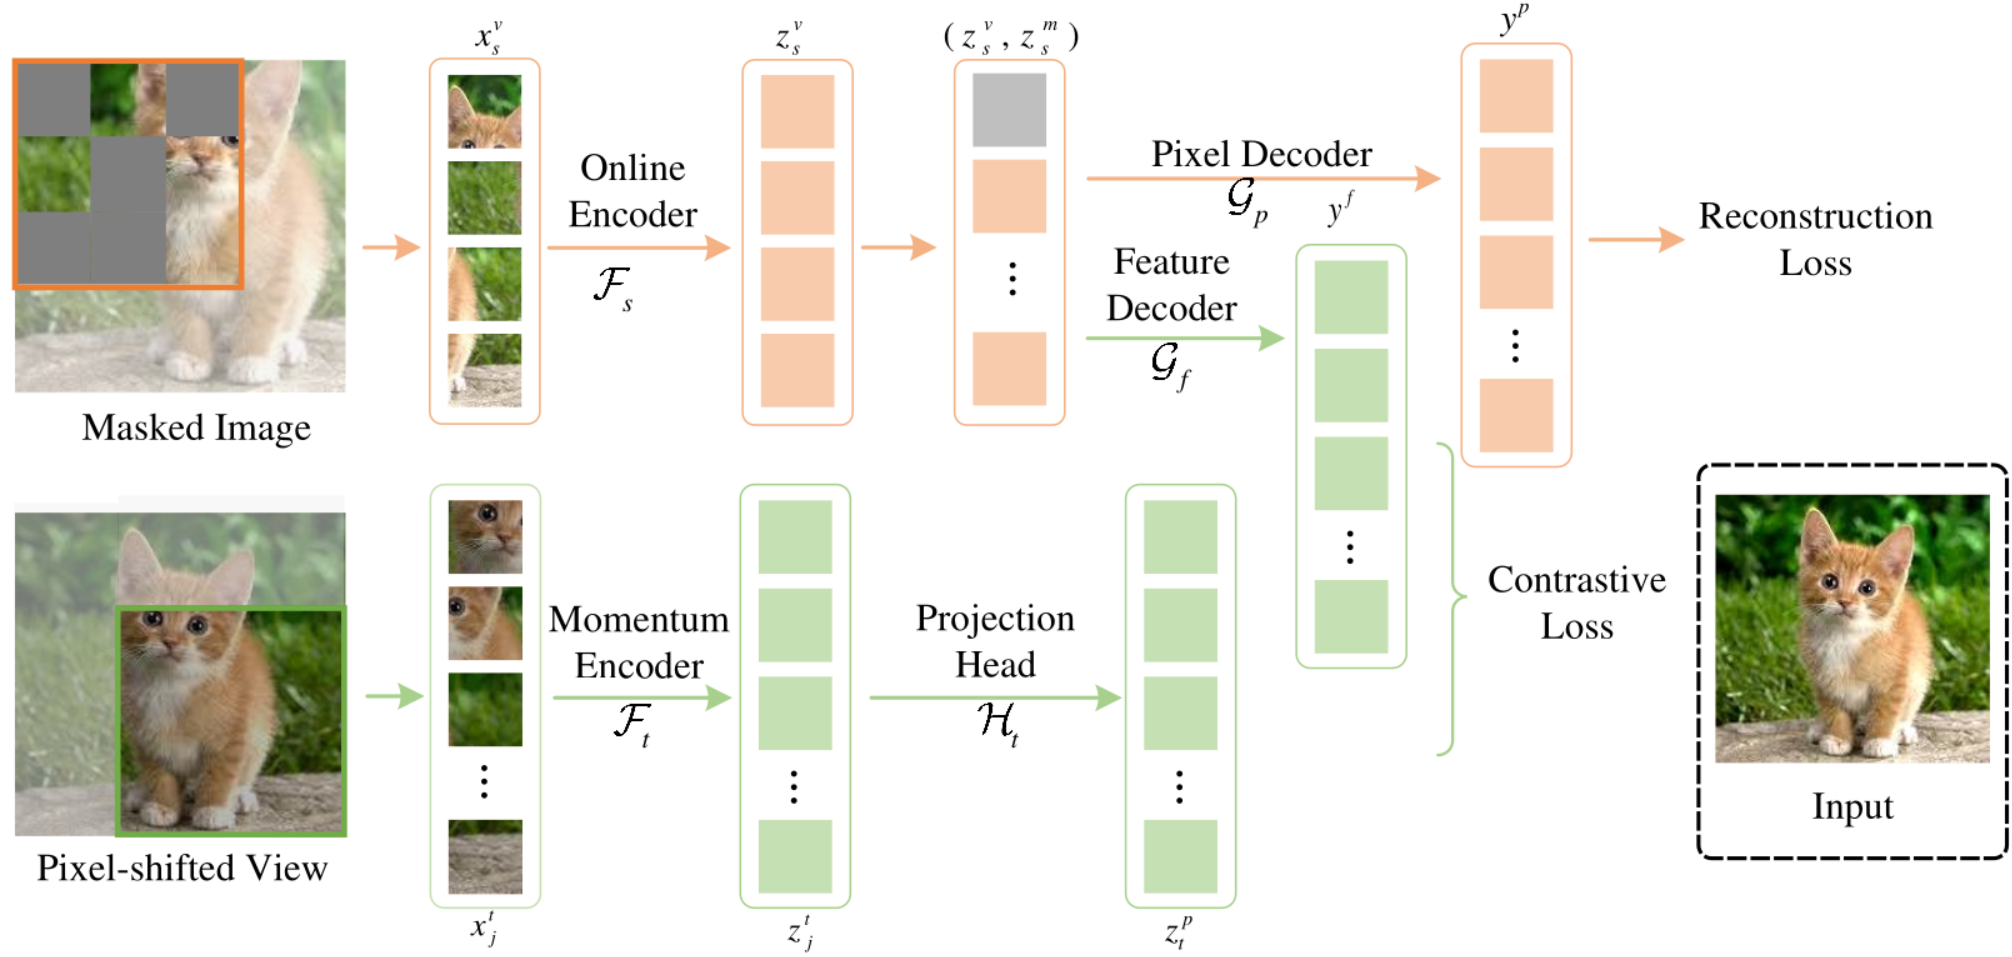
\includegraphics[width=0.7\textwidth]{src/CMAE.png}
  \centering
  \caption{CMAE 模型架構圖。\\圖片來源:https://arxiv.org/pdf/2207.13532}
  \label{fig:CMAE-architecture}
\end{figure}

\subsubsection{Finetune 模型}
在微調的階段,我參考學姐的論文,一樣使用 ViT 作為分類器的骨幹架構。具體來說,將預訓練得到的 encoder 權重載入到 ViT 模型中,將輸出進行全局平均池化以獲取全局特徵。接下來加入一個全連接層(Fully Connected Layer, FC)來進行 PD-L1 表現的預測。這樣的設計能夠充分利用預訓練階段學到的特徵表示,並且在微調階段進行針對性的調整以適應 PD-L1 分類任務。

以下是微調階段的模型架構:
\begin{figure}[H]
  \centering
  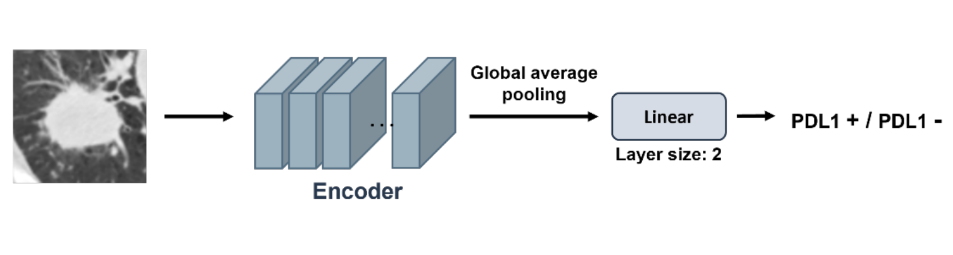
\includegraphics[width=0.8\textwidth]{src/finetune.png}
  \centering
  \caption{Finetune 模型架構圖。\\圖片來源:周姵妤學姐碩士論文}
  \label{fig:finetune-architecture}
\end{figure}


\subsection{性能指標}

在判斷模型的預測效能時,我們將使用以下指標進行評估:
正確率(Accuracy)、靈敏度(Sensitivity)、  特異度(Specificity)與 AUC(Area under curve),
而這些指標的計算方式可由混淆矩陣得出(Confusion Matrix)得出,具體的混淆矩陣可分為四個象限:
\begin{itemize}
    \item 真陽性(True Positive, TP):模型正確預測為陽性的數量。
    \item 假陽性(False Positive, FP):模型錯誤預測為陽性的數量。
    \item 真陰性(True Negative, TN):模型正確預測為陰性的數量。
    \item 假陰性(False Negative, FN):模型錯誤預測為陰性的數量。
\end{itemize}

在本專題中,我們稍微修改了混淆矩陣的定義,
將陽性定義為 PD-L1 表現高於 50\% 的患者,陰性則為低於 50\% 的患者。

\begin{table}[h]
\centering
\begin{tabular}{|c|c|c|}
\hline
 & \textbf{實際陽性} & \textbf{實際陰性} \\ \hline
\textbf{預測陽性} & TP & FP \\ \hline
\textbf{預測陰性} & FN & TN \\ \hline
\end{tabular}
\caption{混淆矩陣}
\end{table}

藉由混淆矩陣,我們可以計算出以下指標:

\subsubsection{正確率(Accuracy)}
正確率是指模型正確預測的比例,在本專題中即正確分辨出 PD-L1 表現高於 50\% 與低於 50\% 的患者比例。
正確率是衡量模型整體預測準確性的指標,
計算公式為:
\begin{equation}
\text{Accuracy} = \frac{TP + TN}{TP + TN + FP + FN}
\end{equation}

\subsubsection{靈敏度(Sensitivity)}
靈敏度(也稱為召回率)是指模型正確預測為陽性的比例。在本專題中,靈敏度即預測 PD-L1 表現高於 50\% 的患者中,實際上也高於 50\% 的比例。
靈敏度是衡量模型對陽性樣本識別能力的指標,
計算公式為:
\begin{equation}
\text{Sensitivity} = \frac{TP}{TP + FN}
\end{equation}

\subsubsection{特異度(Specificity)}
特異度是指模型正確預測為陰性的比例。在本專題中,特異度即預測 PD-L1 表現低於 50\% 的患者中,實際上也低於 50\% 的比例。
特異度是衡量模型對陰性樣本識別能力的指標,
計算公式為:
\begin{equation}
\text{Specificity} = \frac{TN}{TN + FP}
\end{equation}
\subsubsection{AUC(Area under curve)}
AUC 是指 ROC 曲線下的面積,ROC 曲線是以假陽性率(False Positive Rate)為橫軸,真陽性率(True Positive Rate)為縱軸所繪製的曲線。
AUC 值介於 0 與 1 之間,值越大表示模型的預測能力越好。
計算公式為:
\begin{equation}
\text{AUC} = \int_{0}^{1} \text{TPR}(FPR) \, d(FPR)
\end{equation}

\begin{figure}[H]
  \centering
  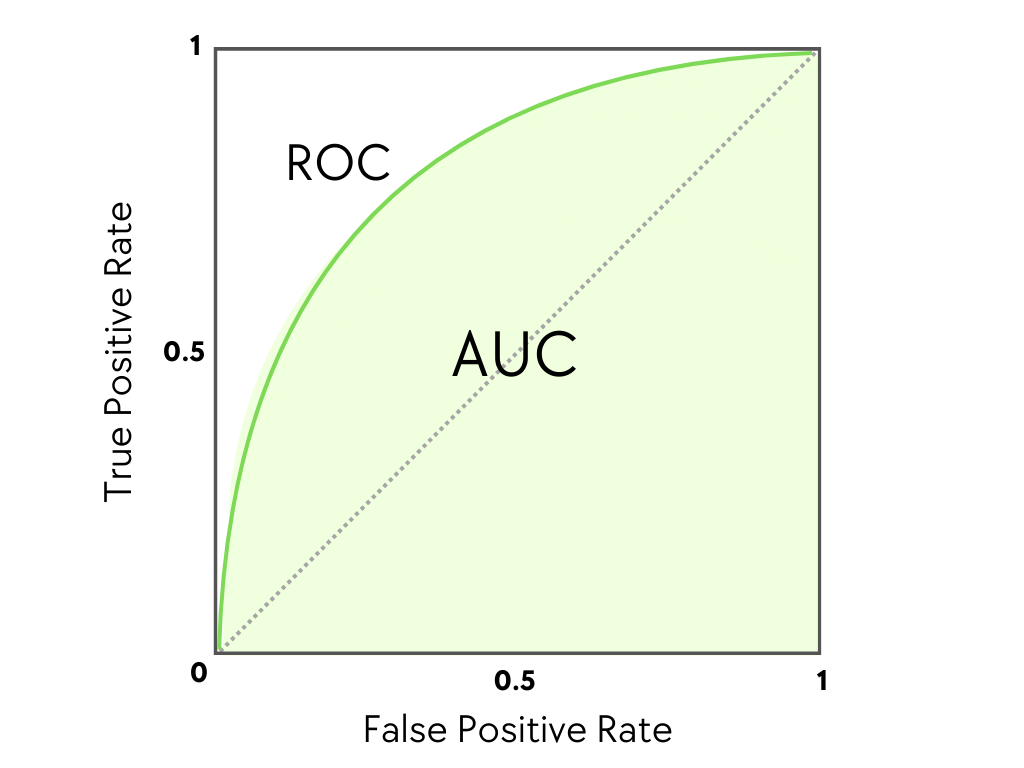
\includegraphics[width=0.5\textwidth]{src/image3.png}
  \centering
  \caption{ROC 曲線及其 AUC 值\\圖片來源:https://www.blog.trainindata.com/auc-roc-analysis/}
  \label{fig:roc-curve}
\end{figure}






\section{研究結果與討論}
在本專題中,由於樣本極度不平衡(陽性:陰性為49:149),因此會以 AUC 作為主要的性能指標。


\subsection{重現 MTMAE 模型}

參考周姵妤學姐的碩士論文,重現 MTMAE 模型的架構與訓練流程。利用 PyTorch 框架實現模型,並使用學姐留下來的 CT 影像與 PD-L1 標記資料進行訓練。
進行 200 個 epoch 的預訓練之後得到 MTMAE 模型的權重,接著使用真實的醫學影像進行微調,並評估模型在 PD-L1 表現預測任務上的準確率。最終多次實驗得到的 AUC 平均值為 0.6168,這個結果與學姐的論文中所報告相差甚遠,推測是因為資料量真的太少,因此不同的排列順序會導致模型的預測結果有很大的差異。


\subsection{加入對比學習模組}
學姐在論文中提到 Quan 等人提出 GCMAE (Global Contrast Masked Autoencoders)的架構,結合 MIM 與對比學習(Contrastive Learning)來學習病理影像的特徵表示。但在本篇論文中,對比學習的模組並未被使用,反而是結合遮罩模型與分割的任務。因此我想嘗試在 MTMAE 模型的基礎上加入對比學習模組,以期提升模型的預測準確率。

\subsubsection{SimLR}
我先是參考了 Chen 等人提出的 SimLR(Simple Linear Regression)對比學習方法,將其應用於 MTMAE 模型中。具體來說,我將在每個訓練 batch 中隨機選擇兩個不同的遮蔽策略,生成兩個不同的影像對,並使用這些影像對進行對比學習。期望能增進模型對語意一致性的建模能力,進而提升 PD-L1 表現預測的準確率。在這部份,嘗試了直接利用 MTMAE 模型訓練出來的 encoder 再繼續使用對比學習模組進行訓練,接著使用此 encoder 進行 finetune,以及直接使用對比學習模組訓練出來的 encoder 進行 finetune,兩種方式進行比較,但兩者的成效都不是很好,尤其是將 MTMAE 模型的 encoder 直接拿來進行對比學習模組訓練,結果甚至比直接使用對比學習模組訓練出來的 encoder 還要差。在訓練的 epoch 數上,我觀察了模型的收斂程度,在單純 simCLR的部份使用了 100 個 epoch,MTMAE 模型預訓練後使用了 10 個 epoch 的微調。結束後使用相同的 finetune 方法進行微調,並評估模型在 PD-L1 表現預測任務上的準確率。

以下是使用 SimLR 方法的實驗結果:

\begin{table}[h]
\centering
\begin{tabular}{lcc}
\toprule
 & \textbf{純粹使用simCLR} & \textbf{MTMAE + SimCLR 微調} \\
\midrule
AUC          & 0.4395 & 0.5000 \\
ACC          & 0.4839 & 0.4355 \\
\bottomrule
\end{tabular}
\caption{SimCLR 方法實驗結果比較}
\label{tab:simclr-results}
\end{table}

使用 simCLR 的效果甚至比亂猜還差,這代表或許純粹的 simCLR 不太適合用於這個任務,結合了 simCLR 的 MTMAE 模型在 PD-L1 表現預測任務上的準確率也並不理想,這或許是因為對比學習的目的與遮罩模型不同,因此破壞了原有的結構。為克服對比學習與遮罩模型的相容問題,我查閱資料後參考了 Huang 等人提出的 CMAE(Contrastive Masked Autoencoders)架構。

\subsubsection{CMAE}
Huang 等人提出了另一個結合對比學習與遮罩模型的 CMAE 架構,這個架構巧妙使用了孿生網路(Siamese Network)結構,將遮罩影像與未遮罩影像進行對比學習。具體來說,我們將輸入影像分成兩個部分,一部分進行遮罩處理,另一部分則不進行遮罩處理,然後將這兩個部分輸入到同一個 encoder 中,最後使用對比損失函數來計算這兩個部分的相似度。這樣的設計能夠有效地學習到影像的全局特徵,同時保留局部細節。然而,CMAE 模型預訓練需要的時間較長,在本專題中來不及完成,因此我先使用 Huang 等人提供的預訓練權重進行微調,並評估模型在 PD-L1 表現預測任務上的準確率。為了驗證其是否有較好的效果,我同時使用 He 等人預訓練好的 MAE 權重進行微調,並比較兩者的效果。CMAE 與 MAE 的預訓練權重皆是在 ImageNet 1k 資料集上進行的。以下是實驗的結果:

\begin{table}[h]
\centering
\begin{tabular}{lcc}
\toprule
 & \textbf{CMAE} & \textbf{MAE} \\
\midrule
AUC          & 0.5625 & 0.5584 \\
ACC          & 0.7419 & 0.6452 \\
\bottomrule
\end{tabular}
\caption{CMAE 方法實驗結果比較}
\label{tab:CMAE-results}
\end{table}

即使 AUC 的表現仍然不太好,但 CMAE 的的成效相較於 MAE 好一些,這或許代表了 CMAE 架構也具有一定的潛力。

\subsection{k-fold 交叉驗證}
原先預計使用 k-fold 模型集成(ensemble)策略來進一步提升模型的預測準確率,但我在操作時出現了一些失誤,原先應該是訓練出 k 個不同的模型,然後將這 k 個模型的預測結果進行平均,但我卻是將同一筆權重進行 k 次微調。這樣反而大大提昇了模型在 test 資料集上的 AUC 表現。我先將訓練的資料分成 5 份,接下來進行 5 輪微調,每輪進行 30 個 epoch,並將其中一份資料作為 validation 資料集,其他四份資料作為training 資料集,其中 validation 資料集不參預權重的更新。將同一筆權重經過五次微調後的  AUC 表現極佳。有思考過是否是因為這樣的方式導致 epoch 數量增加,因此模型才有更好的表現。於是我使用原本的 finetune 方法,將同一筆權重進行 150 個 epoch 的微調,結果發現 AUC 表現較差。我也考慮到是否是因為 learning rate 並沒有在每一輪中重置,因此我又進行了一次實驗:在 5 輪微調中將資料固定,效果一樣較差。查閱資料後發現似乎沒有類似的論文,但這或許跟機器學習中的遺忘機制有關系,在神經網路中,有時會隨機遮罩一部分的權重,使其在訓練過程中不斷更新,這樣能夠避免模型過擬合到某一個特定的資料集。或許這樣的方式能夠讓模型在每一輪微調中都能夠學習到新的特徵表示,進而提升模型的預測準確率。


\begin{table}[h]
\centering
\begin{tabular}{lccc}
\toprule
 & \textbf{5-fold(輪流遮住資料)} & \textbf{5-fold(訓練資料固定} & \textbf{150 個 epoch} \\
\midrule
AUC          & 0.6984 & 0.5645 & 0.6644\\
ACC         & 00.7419 & 0.5421 & 0.7419\\
\bottomrule
\end{tabular}
\caption{5-fold 方法實驗結果比較}
\label{tab:5-fold-results}
\end{table}

\newpage

\section{結論與展望}
在本專題中,我嘗試還原了周姵妤學姐的碩士論文中提出的 MTMAE 模型,並在此基礎上進行改良。通過加入對比學習模組與模型集成策略,我期望能夠進一步提升 PD-L1 表現預測的準確率。實驗結果顯示,MTMAE 模型在 PD-L1 表現預測任務上具有良好的性能,特別是在資料量不足的情況下,模型仍能夠達到較高的 AUC 值。我嘗試了 SimLR 的方法,發現直接以 MTMAE 模型的預訓練權重進行對比學習的效果並不理想,這或許是對比學習的目的與遮罩模型不同,因此破壞了員有的結構。接著,我嘗試了 CMAE 的方法,但由於其預訓練需要的時間較長,在本專題中來不及完成,因此我先使用 Huang 等人提供的預訓練權重進行微調,並評估模型在 PD-L1 表現預測任務上的準確率。最後,我使用類似 k-fold 模型集成策略進行微調,發現其 AUC 表現極佳,這或許是因為模型在每一輪微調中都能夠學習到新的特徵表示,進而提升模型的預測準確率。

在這短短兩個月中,我從幾乎不了解神經網路的基本概念,到能夠使用 PyTorch 框架實現 MTMAE 模型,並在此基礎上進行改良,這是我在這次專題中最大的收穫。同時,也為了解決問題而去閱讀了許多相關的論文與資料,這讓我對自監督學習、對比學習與模型集成有了更深入的了解。雖然時間有限,但我仍然學到了很多關於機器學習的知識,這些知識將對我未來的研究與學習有很大的幫助。目前思考了幾個未來可能嘗試的方向:

\begin{enumerate}
  \item 使用完整的 CMAE 模型進行預訓練,並評估其在 PD-L1 表現預測任務上的準確率。
  \item 將 MTMAE 架構中提出的分割任務加入 CMAE 的架構中,結合分割任務、對比學習、遮罩模型與分類任務,進一步提升模型的表徵學習能力。
  \item 讓模型不再僅判斷正負,而是將 PD-L1 表現分成三個等級:高表現(>50\%)、中表現(20\%~50\%)與低表現(<20\%),更細緻地預測 PD-L1 的表現。
  \item 嘗試將正確的 k-fold 模型集成策略應用於微調階段,將多個不同的模型進行集成,進一步提升模型的預測準確率。
\end{enumerate}

\section{參考文獻}
\begin{enumerate}
    \item 周姵妤,肺部電腦斷層掃描之非小細胞癌 PD-L1 表現預測 :結合遮蓋圖像模型與生成對抗網路,碩士論文,國立臺灣大學,2024。
    \item Devlin, Jacob, et al. "Bert: Pre-training of deep bidirectional transformers for language understanding." Proceedings of the 2019 conference of the North American chapter of the association for computational linguistics: human language technologies, volume 1 (long and short papers). 2019.
    \item Bao, Hangbo, et al. "Beit: Bert pre-training of image transformers." arXiv preprint arXiv:2106.08254 (2021).
    \item He, Kaiming, et al. "Masked autoencoders are scalable vision learners." Proceedings of the IEEE/CVF conference on computer vision and pattern recognition. 2022.
    \item Chen, Ting, et al. "A simple framework for contrastive learning of visual representations." International conference on machine learning. PmLR, 2020.
    \item Quan, Hao, et al. "Global contrast-masked autoencoders are powerful pathological representation learners." Pattern Recognition 156 (2024): 110745.
    \item Huang, Zhicheng, et al. "Contrastive masked autoencoders are stronger vision learners." IEEE Transactions on Pattern Analysis and Machine Intelligence 46.4 (2023): 2506-2517.
\end{enumerate}

\end{document}